

\tikzset{every picture/.style={line width=0.75pt}} %set default line width to 0.75pt        

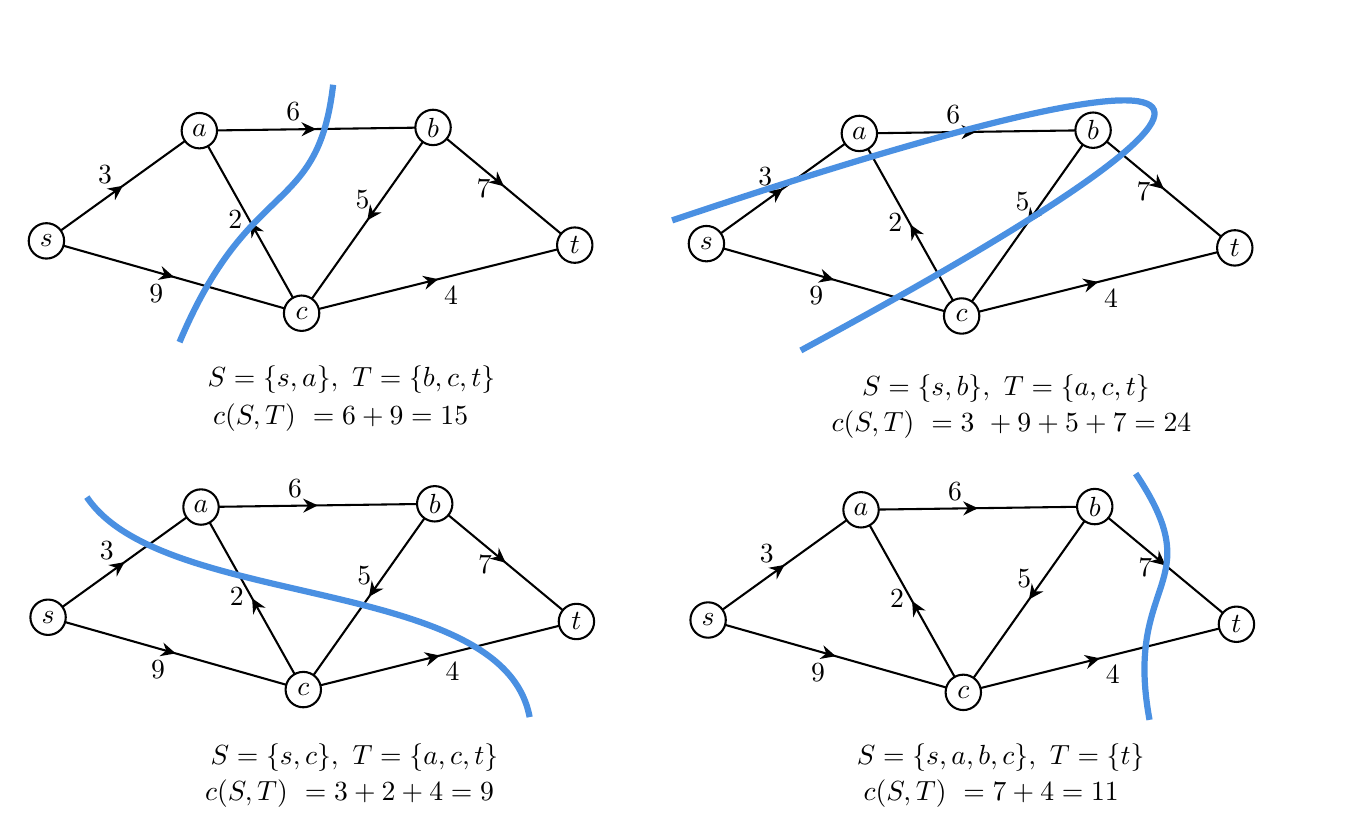
\begin{tikzpicture}[x=0.5pt,y=0.5pt,yscale=-1,xscale=1]
%uncomment if require: \path (0,536); %set diagram left start at 0, and has height of 536

%Straight Lines [id:da23489693411656742] 
\draw    (227.22,173.11) -- (322.22,38.84) ;
\draw [shift={(274.72,105.98)}, rotate = 305.28] [fill={rgb, 255:red, 0; green, 0; blue, 0 }  ][line width=0.08]  [draw opacity=0] (10.72,-5.15) -- (0,0) -- (10.72,5.15) -- (7.12,0) -- cycle    ;
%Straight Lines [id:da09676480347323557] 
\draw    (153.31,41.18) -- (227.22,173.11) ;
\draw [shift={(190.27,107.14)}, rotate = 60.74] [fill={rgb, 255:red, 0; green, 0; blue, 0 }  ][line width=0.08]  [draw opacity=0] (10.72,-5.15) -- (0,0) -- (10.72,5.15) -- (7.12,0) -- cycle    ;
%Straight Lines [id:da7496187873279541] 
\draw    (42.79,120.83) -- (227.22,173.11) ;
\draw [shift={(135.01,146.97)}, rotate = 195.83] [fill={rgb, 255:red, 0; green, 0; blue, 0 }  ][line width=0.08]  [draw opacity=0] (10.72,-5.15) -- (0,0) -- (10.72,5.15) -- (7.12,0) -- cycle    ;
%Straight Lines [id:da6471652125495851] 
\draw    (424.62,123.9) -- (227.22,173.11) ;
\draw [shift={(325.92,148.5)}, rotate = 166] [fill={rgb, 255:red, 0; green, 0; blue, 0 }  ][line width=0.08]  [draw opacity=0] (10.72,-5.15) -- (0,0) -- (10.72,5.15) -- (7.12,0) -- cycle    ;
%Straight Lines [id:da7396594464148104] 
\draw    (42.79,120.83) -- (153.31,41.18) ;
\draw [shift={(98.05,81)}, rotate = 144.22] [fill={rgb, 255:red, 0; green, 0; blue, 0 }  ][line width=0.08]  [draw opacity=0] (10.72,-5.15) -- (0,0) -- (10.72,5.15) -- (7.12,0) -- cycle    ;
%Straight Lines [id:da8785496993916957] 
\draw    (322.22,38.84) -- (424.62,123.9) ;
\draw [shift={(373.42,81.37)}, rotate = 219.71] [fill={rgb, 255:red, 0; green, 0; blue, 0 }  ][line width=0.08]  [draw opacity=0] (10.72,-5.15) -- (0,0) -- (10.72,5.15) -- (7.12,0) -- cycle    ;
%Straight Lines [id:da034251061287473794] 
\draw    (153.31,41.18) -- (322.22,38.84) ;
\draw [shift={(237.76,40.01)}, rotate = 179.21] [fill={rgb, 255:red, 0; green, 0; blue, 0 }  ][line width=0.08]  [draw opacity=0] (10.72,-5.15) -- (0,0) -- (10.72,5.15) -- (7.12,0) -- cycle    ;
%Shape: Ellipse [id:dp13275608995798827] 
\draw  [fill={rgb, 255:red, 255; green, 255; blue, 255 }  ,fill opacity=1 ] (30,120.83) .. controls (30,113.77) and (35.73,108.04) .. (42.79,108.04) .. controls (49.86,108.04) and (55.58,113.77) .. (55.58,120.83) .. controls (55.58,127.9) and (49.86,133.62) .. (42.79,133.62) .. controls (35.73,133.62) and (30,127.9) .. (30,120.83) -- cycle ;
%Shape: Ellipse [id:dp2393540854923375] 
\draw  [fill={rgb, 255:red, 255; green, 255; blue, 255 }  ,fill opacity=1 ] (140.52,41.18) .. controls (140.52,34.11) and (146.25,28.39) .. (153.31,28.39) .. controls (160.38,28.39) and (166.1,34.11) .. (166.1,41.18) .. controls (166.1,48.24) and (160.38,53.97) .. (153.31,53.97) .. controls (146.25,53.97) and (140.52,48.24) .. (140.52,41.18) -- cycle ;
%Shape: Ellipse [id:dp7789774005093756] 
\draw  [fill={rgb, 255:red, 255; green, 255; blue, 255 }  ,fill opacity=1 ] (309.43,38.84) .. controls (309.43,31.78) and (315.15,26.05) .. (322.22,26.05) .. controls (329.28,26.05) and (335.01,31.78) .. (335.01,38.84) .. controls (335.01,45.9) and (329.28,51.63) .. (322.22,51.63) .. controls (315.15,51.63) and (309.43,45.9) .. (309.43,38.84) -- cycle ;
%Shape: Ellipse [id:dp8802069759302812] 
\draw  [fill={rgb, 255:red, 255; green, 255; blue, 255 }  ,fill opacity=1 ] (214.43,173.11) .. controls (214.43,166.05) and (220.15,160.32) .. (227.22,160.32) .. controls (234.28,160.32) and (240.01,166.05) .. (240.01,173.11) .. controls (240.01,180.18) and (234.28,185.9) .. (227.22,185.9) .. controls (220.15,185.9) and (214.43,180.18) .. (214.43,173.11) -- cycle ;
%Shape: Ellipse [id:dp9822973935357934] 
\draw  [fill={rgb, 255:red, 255; green, 255; blue, 255 }  ,fill opacity=1 ] (411.83,123.9) .. controls (411.83,116.83) and (417.56,111.11) .. (424.62,111.11) .. controls (431.69,111.11) and (437.41,116.83) .. (437.41,123.9) .. controls (437.41,130.96) and (431.69,136.69) .. (424.62,136.69) .. controls (417.56,136.69) and (411.83,130.96) .. (411.83,123.9) -- cycle ;
%Straight Lines [id:da9658635220732651] 
\draw    (704.22,175.11) -- (799.22,40.84) ;
\draw [shift={(751.72,107.98)}, rotate = 305.28] [fill={rgb, 255:red, 0; green, 0; blue, 0 }  ][line width=0.08]  [draw opacity=0] (10.72,-5.15) -- (0,0) -- (10.72,5.15) -- (7.12,0) -- cycle    ;
%Straight Lines [id:da82351979522789] 
\draw    (630.31,43.18) -- (704.22,175.11) ;
\draw [shift={(667.27,109.14)}, rotate = 60.74] [fill={rgb, 255:red, 0; green, 0; blue, 0 }  ][line width=0.08]  [draw opacity=0] (10.72,-5.15) -- (0,0) -- (10.72,5.15) -- (7.12,0) -- cycle    ;
%Straight Lines [id:da7840831624948497] 
\draw    (519.79,122.83) -- (704.22,175.11) ;
\draw [shift={(612.01,148.97)}, rotate = 195.83] [fill={rgb, 255:red, 0; green, 0; blue, 0 }  ][line width=0.08]  [draw opacity=0] (10.72,-5.15) -- (0,0) -- (10.72,5.15) -- (7.12,0) -- cycle    ;
%Straight Lines [id:da14276151552176897] 
\draw    (901.62,125.9) -- (704.22,175.11) ;
\draw [shift={(802.92,150.5)}, rotate = 166] [fill={rgb, 255:red, 0; green, 0; blue, 0 }  ][line width=0.08]  [draw opacity=0] (10.72,-5.15) -- (0,0) -- (10.72,5.15) -- (7.12,0) -- cycle    ;
%Straight Lines [id:da14209561142628646] 
\draw    (519.79,122.83) -- (630.31,43.18) ;
\draw [shift={(575.05,83)}, rotate = 144.22] [fill={rgb, 255:red, 0; green, 0; blue, 0 }  ][line width=0.08]  [draw opacity=0] (10.72,-5.15) -- (0,0) -- (10.72,5.15) -- (7.12,0) -- cycle    ;
%Straight Lines [id:da8871601533202532] 
\draw    (799.22,40.84) -- (901.62,125.9) ;
\draw [shift={(850.42,83.37)}, rotate = 219.71] [fill={rgb, 255:red, 0; green, 0; blue, 0 }  ][line width=0.08]  [draw opacity=0] (10.72,-5.15) -- (0,0) -- (10.72,5.15) -- (7.12,0) -- cycle    ;
%Straight Lines [id:da23862638545176929] 
\draw    (630.31,43.18) -- (799.22,40.84) ;
\draw [shift={(714.76,42.01)}, rotate = 179.21] [fill={rgb, 255:red, 0; green, 0; blue, 0 }  ][line width=0.08]  [draw opacity=0] (10.72,-5.15) -- (0,0) -- (10.72,5.15) -- (7.12,0) -- cycle    ;
%Shape: Ellipse [id:dp48467109777209416] 
\draw  [fill={rgb, 255:red, 255; green, 255; blue, 255 }  ,fill opacity=1 ] (507,122.83) .. controls (507,115.77) and (512.73,110.04) .. (519.79,110.04) .. controls (526.86,110.04) and (532.58,115.77) .. (532.58,122.83) .. controls (532.58,129.9) and (526.86,135.62) .. (519.79,135.62) .. controls (512.73,135.62) and (507,129.9) .. (507,122.83) -- cycle ;
%Shape: Ellipse [id:dp9425702686922498] 
\draw  [fill={rgb, 255:red, 255; green, 255; blue, 255 }  ,fill opacity=1 ] (617.52,43.18) .. controls (617.52,36.11) and (623.25,30.39) .. (630.31,30.39) .. controls (637.38,30.39) and (643.1,36.11) .. (643.1,43.18) .. controls (643.1,50.24) and (637.38,55.97) .. (630.31,55.97) .. controls (623.25,55.97) and (617.52,50.24) .. (617.52,43.18) -- cycle ;
%Shape: Ellipse [id:dp6055322842292827] 
\draw  [fill={rgb, 255:red, 255; green, 255; blue, 255 }  ,fill opacity=1 ] (786.43,40.84) .. controls (786.43,33.78) and (792.15,28.05) .. (799.22,28.05) .. controls (806.28,28.05) and (812.01,33.78) .. (812.01,40.84) .. controls (812.01,47.9) and (806.28,53.63) .. (799.22,53.63) .. controls (792.15,53.63) and (786.43,47.9) .. (786.43,40.84) -- cycle ;
%Shape: Ellipse [id:dp03377296854096312] 
\draw  [fill={rgb, 255:red, 255; green, 255; blue, 255 }  ,fill opacity=1 ] (691.43,175.11) .. controls (691.43,168.05) and (697.15,162.32) .. (704.22,162.32) .. controls (711.28,162.32) and (717.01,168.05) .. (717.01,175.11) .. controls (717.01,182.18) and (711.28,187.9) .. (704.22,187.9) .. controls (697.15,187.9) and (691.43,182.18) .. (691.43,175.11) -- cycle ;
%Shape: Ellipse [id:dp3350053760321048] 
\draw  [fill={rgb, 255:red, 255; green, 255; blue, 255 }  ,fill opacity=1 ] (888.83,125.9) .. controls (888.83,118.83) and (894.56,113.11) .. (901.62,113.11) .. controls (908.69,113.11) and (914.41,118.83) .. (914.41,125.9) .. controls (914.41,132.96) and (908.69,138.69) .. (901.62,138.69) .. controls (894.56,138.69) and (888.83,132.96) .. (888.83,125.9) -- cycle ;
%Curve Lines [id:da21781374711830293] 
\draw [color={rgb, 255:red, 74; green, 144; blue, 226 }  ,draw opacity=1 ][line width=2.25]    (250,8) .. controls (239,104) and (190,73) .. (139,194) ;
%Curve Lines [id:da975003782049386] 
\draw [color={rgb, 255:red, 74; green, 144; blue, 226 }  ,draw opacity=1 ][line width=2.25]    (495,106) .. controls (903,-31) and (977,-10) .. (588,200) ;
%Straight Lines [id:da8822105936811906] 
\draw    (228.43,445.11) -- (323.42,310.84) ;
\draw [shift={(275.92,377.98)}, rotate = 305.28] [fill={rgb, 255:red, 0; green, 0; blue, 0 }  ][line width=0.08]  [draw opacity=0] (10.72,-5.15) -- (0,0) -- (10.72,5.15) -- (7.12,0) -- cycle    ;
%Straight Lines [id:da8763249151085379] 
\draw    (154.52,313.18) -- (228.43,445.11) ;
\draw [shift={(191.47,379.14)}, rotate = 60.74] [fill={rgb, 255:red, 0; green, 0; blue, 0 }  ][line width=0.08]  [draw opacity=0] (10.72,-5.15) -- (0,0) -- (10.72,5.15) -- (7.12,0) -- cycle    ;
%Straight Lines [id:da09137103175509198] 
\draw    (44,392.83) -- (228.43,445.11) ;
\draw [shift={(136.21,418.97)}, rotate = 195.83] [fill={rgb, 255:red, 0; green, 0; blue, 0 }  ][line width=0.08]  [draw opacity=0] (10.72,-5.15) -- (0,0) -- (10.72,5.15) -- (7.12,0) -- cycle    ;
%Straight Lines [id:da5294224641432785] 
\draw    (425.83,395.9) -- (228.43,445.11) ;
\draw [shift={(327.13,420.5)}, rotate = 166] [fill={rgb, 255:red, 0; green, 0; blue, 0 }  ][line width=0.08]  [draw opacity=0] (10.72,-5.15) -- (0,0) -- (10.72,5.15) -- (7.12,0) -- cycle    ;
%Straight Lines [id:da9311120593906992] 
\draw    (44,392.83) -- (154.52,313.18) ;
\draw [shift={(99.26,353)}, rotate = 144.22] [fill={rgb, 255:red, 0; green, 0; blue, 0 }  ][line width=0.08]  [draw opacity=0] (10.72,-5.15) -- (0,0) -- (10.72,5.15) -- (7.12,0) -- cycle    ;
%Straight Lines [id:da003018118529787839] 
\draw    (323.42,310.84) -- (425.83,395.9) ;
\draw [shift={(374.63,353.37)}, rotate = 219.71] [fill={rgb, 255:red, 0; green, 0; blue, 0 }  ][line width=0.08]  [draw opacity=0] (10.72,-5.15) -- (0,0) -- (10.72,5.15) -- (7.12,0) -- cycle    ;
%Straight Lines [id:da33441362774690564] 
\draw    (154.52,313.18) -- (323.42,310.84) ;
\draw [shift={(238.97,312.01)}, rotate = 179.21] [fill={rgb, 255:red, 0; green, 0; blue, 0 }  ][line width=0.08]  [draw opacity=0] (10.72,-5.15) -- (0,0) -- (10.72,5.15) -- (7.12,0) -- cycle    ;
%Shape: Ellipse [id:dp5180015708462345] 
\draw  [fill={rgb, 255:red, 255; green, 255; blue, 255 }  ,fill opacity=1 ] (31.21,392.83) .. controls (31.21,385.77) and (36.94,380.04) .. (44,380.04) .. controls (51.06,380.04) and (56.79,385.77) .. (56.79,392.83) .. controls (56.79,399.9) and (51.06,405.62) .. (44,405.62) .. controls (36.94,405.62) and (31.21,399.9) .. (31.21,392.83) -- cycle ;
%Shape: Ellipse [id:dp6316874948701398] 
\draw  [fill={rgb, 255:red, 255; green, 255; blue, 255 }  ,fill opacity=1 ] (141.73,313.18) .. controls (141.73,306.11) and (147.46,300.39) .. (154.52,300.39) .. controls (161.58,300.39) and (167.31,306.11) .. (167.31,313.18) .. controls (167.31,320.24) and (161.58,325.97) .. (154.52,325.97) .. controls (147.46,325.97) and (141.73,320.24) .. (141.73,313.18) -- cycle ;
%Shape: Ellipse [id:dp3057393329033985] 
\draw  [fill={rgb, 255:red, 255; green, 255; blue, 255 }  ,fill opacity=1 ] (310.63,310.84) .. controls (310.63,303.78) and (316.36,298.05) .. (323.42,298.05) .. controls (330.49,298.05) and (336.21,303.78) .. (336.21,310.84) .. controls (336.21,317.9) and (330.49,323.63) .. (323.42,323.63) .. controls (316.36,323.63) and (310.63,317.9) .. (310.63,310.84) -- cycle ;
%Shape: Ellipse [id:dp44953504280435763] 
\draw  [fill={rgb, 255:red, 255; green, 255; blue, 255 }  ,fill opacity=1 ] (215.64,445.11) .. controls (215.64,438.05) and (221.36,432.32) .. (228.43,432.32) .. controls (235.49,432.32) and (241.22,438.05) .. (241.22,445.11) .. controls (241.22,452.18) and (235.49,457.9) .. (228.43,457.9) .. controls (221.36,457.9) and (215.64,452.18) .. (215.64,445.11) -- cycle ;
%Shape: Ellipse [id:dp48843863247887387] 
\draw  [fill={rgb, 255:red, 255; green, 255; blue, 255 }  ,fill opacity=1 ] (413.04,395.9) .. controls (413.04,388.83) and (418.77,383.11) .. (425.83,383.11) .. controls (432.89,383.11) and (438.62,388.83) .. (438.62,395.9) .. controls (438.62,402.96) and (432.89,408.69) .. (425.83,408.69) .. controls (418.77,408.69) and (413.04,402.96) .. (413.04,395.9) -- cycle ;
%Straight Lines [id:da27790436141665653] 
\draw    (705.43,447.11) -- (800.42,312.84) ;
\draw [shift={(752.92,379.98)}, rotate = 305.28] [fill={rgb, 255:red, 0; green, 0; blue, 0 }  ][line width=0.08]  [draw opacity=0] (10.72,-5.15) -- (0,0) -- (10.72,5.15) -- (7.12,0) -- cycle    ;
%Straight Lines [id:da5721790090964675] 
\draw    (631.52,315.18) -- (705.43,447.11) ;
\draw [shift={(668.47,381.14)}, rotate = 60.74] [fill={rgb, 255:red, 0; green, 0; blue, 0 }  ][line width=0.08]  [draw opacity=0] (10.72,-5.15) -- (0,0) -- (10.72,5.15) -- (7.12,0) -- cycle    ;
%Straight Lines [id:da6894877787879099] 
\draw    (521,394.83) -- (705.43,447.11) ;
\draw [shift={(613.21,420.97)}, rotate = 195.83] [fill={rgb, 255:red, 0; green, 0; blue, 0 }  ][line width=0.08]  [draw opacity=0] (10.72,-5.15) -- (0,0) -- (10.72,5.15) -- (7.12,0) -- cycle    ;
%Straight Lines [id:da4557406380885568] 
\draw    (902.83,397.9) -- (705.43,447.11) ;
\draw [shift={(804.13,422.5)}, rotate = 166] [fill={rgb, 255:red, 0; green, 0; blue, 0 }  ][line width=0.08]  [draw opacity=0] (10.72,-5.15) -- (0,0) -- (10.72,5.15) -- (7.12,0) -- cycle    ;
%Straight Lines [id:da19240359352418468] 
\draw    (521,394.83) -- (631.52,315.18) ;
\draw [shift={(576.26,355)}, rotate = 144.22] [fill={rgb, 255:red, 0; green, 0; blue, 0 }  ][line width=0.08]  [draw opacity=0] (10.72,-5.15) -- (0,0) -- (10.72,5.15) -- (7.12,0) -- cycle    ;
%Straight Lines [id:da9215059687189877] 
\draw    (800.42,312.84) -- (902.83,397.9) ;
\draw [shift={(851.63,355.37)}, rotate = 219.71] [fill={rgb, 255:red, 0; green, 0; blue, 0 }  ][line width=0.08]  [draw opacity=0] (10.72,-5.15) -- (0,0) -- (10.72,5.15) -- (7.12,0) -- cycle    ;
%Straight Lines [id:da44324187024067707] 
\draw    (631.52,315.18) -- (800.42,312.84) ;
\draw [shift={(715.97,314.01)}, rotate = 179.21] [fill={rgb, 255:red, 0; green, 0; blue, 0 }  ][line width=0.08]  [draw opacity=0] (10.72,-5.15) -- (0,0) -- (10.72,5.15) -- (7.12,0) -- cycle    ;
%Shape: Ellipse [id:dp9279471109735129] 
\draw  [fill={rgb, 255:red, 255; green, 255; blue, 255 }  ,fill opacity=1 ] (508.21,394.83) .. controls (508.21,387.77) and (513.94,382.04) .. (521,382.04) .. controls (528.06,382.04) and (533.79,387.77) .. (533.79,394.83) .. controls (533.79,401.9) and (528.06,407.62) .. (521,407.62) .. controls (513.94,407.62) and (508.21,401.9) .. (508.21,394.83) -- cycle ;
%Shape: Ellipse [id:dp3102644915033731] 
\draw  [fill={rgb, 255:red, 255; green, 255; blue, 255 }  ,fill opacity=1 ] (618.73,315.18) .. controls (618.73,308.11) and (624.46,302.39) .. (631.52,302.39) .. controls (638.58,302.39) and (644.31,308.11) .. (644.31,315.18) .. controls (644.31,322.24) and (638.58,327.97) .. (631.52,327.97) .. controls (624.46,327.97) and (618.73,322.24) .. (618.73,315.18) -- cycle ;
%Shape: Ellipse [id:dp9763670676011375] 
\draw  [fill={rgb, 255:red, 255; green, 255; blue, 255 }  ,fill opacity=1 ] (787.63,312.84) .. controls (787.63,305.78) and (793.36,300.05) .. (800.42,300.05) .. controls (807.49,300.05) and (813.21,305.78) .. (813.21,312.84) .. controls (813.21,319.9) and (807.49,325.63) .. (800.42,325.63) .. controls (793.36,325.63) and (787.63,319.9) .. (787.63,312.84) -- cycle ;
%Shape: Ellipse [id:dp18226709096578564] 
\draw  [fill={rgb, 255:red, 255; green, 255; blue, 255 }  ,fill opacity=1 ] (692.64,447.11) .. controls (692.64,440.05) and (698.36,434.32) .. (705.43,434.32) .. controls (712.49,434.32) and (718.22,440.05) .. (718.22,447.11) .. controls (718.22,454.18) and (712.49,459.9) .. (705.43,459.9) .. controls (698.36,459.9) and (692.64,454.18) .. (692.64,447.11) -- cycle ;
%Shape: Ellipse [id:dp6076949162731399] 
\draw  [fill={rgb, 255:red, 255; green, 255; blue, 255 }  ,fill opacity=1 ] (890.04,397.9) .. controls (890.04,390.83) and (895.77,385.11) .. (902.83,385.11) .. controls (909.89,385.11) and (915.62,390.83) .. (915.62,397.9) .. controls (915.62,404.96) and (909.89,410.69) .. (902.83,410.69) .. controls (895.77,410.69) and (890.04,404.96) .. (890.04,397.9) -- cycle ;
%Curve Lines [id:da22541217186849039] 
\draw [color={rgb, 255:red, 74; green, 144; blue, 226 }  ,draw opacity=1 ][line width=2.25]    (72,306) .. controls (127,388) and (373,362) .. (392,465) ;
%Curve Lines [id:da31049024409298764] 
\draw [color={rgb, 255:red, 74; green, 144; blue, 226 }  ,draw opacity=1 ][line width=2.25]    (830,289) .. controls (885,371) and (821,364) .. (840,467) ;

% Text Node
\draw (42.79,120.83) node   [align=left] {$\displaystyle s$};
% Text Node
\draw (153.31,41.18) node   [align=left] {$\displaystyle a$};
% Text Node
\draw (322.22,38.84) node   [align=left] {$\displaystyle b$};
% Text Node
\draw (227.22,173.11) node   [align=left] {$\displaystyle c$};
% Text Node
\draw (424.62,123.9) node   [align=left] {$\displaystyle t$};
% Text Node
\draw (115,150) node [anchor=north west][inner sep=0.75pt]   [align=left] {$\displaystyle 9$};
% Text Node
\draw (264,82) node [anchor=north west][inner sep=0.75pt]   [align=left] {$\displaystyle 5$};
% Text Node
\draw (172,97) node [anchor=north west][inner sep=0.75pt]   [align=left] {$\displaystyle 2$};
% Text Node
\draw (78,64) node [anchor=north west][inner sep=0.75pt]   [align=left] {$\displaystyle 3$};
% Text Node
\draw (327.92,151.5) node [anchor=north west][inner sep=0.75pt]   [align=left] {$\displaystyle 4$};
% Text Node
\draw (351.42,74.37) node [anchor=north west][inner sep=0.75pt]   [align=left] {$\displaystyle 7$};
% Text Node
\draw (214,19) node [anchor=north west][inner sep=0.75pt]   [align=left] {$\displaystyle 6$};
% Text Node
\draw (161,236) node [anchor=north west][inner sep=0.75pt]   [align=left] {$\displaystyle c( S,T) \ =6+9=15$};
% Text Node
\draw (157,209) node [anchor=north west][inner sep=0.75pt]   [align=left] {$\displaystyle S=\{s,a\} ,\ T=\{b,c,t\}$};
% Text Node
\draw (519.79,122.83) node   [align=left] {$\displaystyle s$};
% Text Node
\draw (630.31,43.18) node   [align=left] {$\displaystyle a$};
% Text Node
\draw (799.22,40.84) node   [align=left] {$\displaystyle b$};
% Text Node
\draw (704.22,175.11) node   [align=left] {$\displaystyle c$};
% Text Node
\draw (901.62,125.9) node   [align=left] {$\displaystyle t$};
% Text Node
\draw (592,152) node [anchor=north west][inner sep=0.75pt]   [align=left] {$\displaystyle 9$};
% Text Node
\draw (741,84) node [anchor=north west][inner sep=0.75pt]   [align=left] {$\displaystyle 5$};
% Text Node
\draw (649,99) node [anchor=north west][inner sep=0.75pt]   [align=left] {$\displaystyle 2$};
% Text Node
\draw (555,66) node [anchor=north west][inner sep=0.75pt]   [align=left] {$\displaystyle 3$};
% Text Node
\draw (804.92,153.5) node [anchor=north west][inner sep=0.75pt]   [align=left] {$\displaystyle 4$};
% Text Node
\draw (828.42,76.37) node [anchor=north west][inner sep=0.75pt]   [align=left] {$\displaystyle 7$};
% Text Node
\draw (691,21) node [anchor=north west][inner sep=0.75pt]   [align=left] {$\displaystyle 6$};
% Text Node
\draw (608,241) node [anchor=north west][inner sep=0.75pt]   [align=left] {$\displaystyle c( S,T) \ =3\ +9+5+7=24$};
% Text Node
\draw (630,215) node [anchor=north west][inner sep=0.75pt]   [align=left] {$\displaystyle S=\{s,b\} ,\ T=\{a,c,t\}$};
% Text Node
\draw (44,392.83) node   [align=left] {$\displaystyle s$};
% Text Node
\draw (154.52,313.18) node   [align=left] {$\displaystyle a$};
% Text Node
\draw (323.42,310.84) node   [align=left] {$\displaystyle b$};
% Text Node
\draw (228.43,445.11) node   [align=left] {$\displaystyle c$};
% Text Node
\draw (425.83,395.9) node   [align=left] {$\displaystyle t$};
% Text Node
\draw (116.21,422) node [anchor=north west][inner sep=0.75pt]   [align=left] {$\displaystyle 9$};
% Text Node
\draw (265.21,354) node [anchor=north west][inner sep=0.75pt]   [align=left] {$\displaystyle 5$};
% Text Node
\draw (173.21,369) node [anchor=north west][inner sep=0.75pt]   [align=left] {$\displaystyle 2$};
% Text Node
\draw (79.21,336) node [anchor=north west][inner sep=0.75pt]   [align=left] {$\displaystyle 3$};
% Text Node
\draw (329.13,423.5) node [anchor=north west][inner sep=0.75pt]   [align=left] {$\displaystyle 4$};
% Text Node
\draw (352.63,346.37) node [anchor=north west][inner sep=0.75pt]   [align=left] {$\displaystyle 7$};
% Text Node
\draw (215.21,291) node [anchor=north west][inner sep=0.75pt]   [align=left] {$\displaystyle 6$};
% Text Node
\draw (155.21,508) node [anchor=north west][inner sep=0.75pt]   [align=left] {$\displaystyle c( S,T) \ =3+2+4=9$};
% Text Node
\draw (159.21,482) node [anchor=north west][inner sep=0.75pt]   [align=left] {$\displaystyle S=\{s,c\} ,\ T=\{a,c,t\}$};
% Text Node
\draw (521,394.83) node   [align=left] {$\displaystyle s$};
% Text Node
\draw (631.52,315.18) node   [align=left] {$\displaystyle a$};
% Text Node
\draw (800.42,312.84) node   [align=left] {$\displaystyle b$};
% Text Node
\draw (705.43,447.11) node   [align=left] {$\displaystyle c$};
% Text Node
\draw (902.83,397.9) node   [align=left] {$\displaystyle t$};
% Text Node
\draw (593.21,424) node [anchor=north west][inner sep=0.75pt]   [align=left] {$\displaystyle 9$};
% Text Node
\draw (742.21,356) node [anchor=north west][inner sep=0.75pt]   [align=left] {$\displaystyle 5$};
% Text Node
\draw (650.21,371) node [anchor=north west][inner sep=0.75pt]   [align=left] {$\displaystyle 2$};
% Text Node
\draw (556.21,338) node [anchor=north west][inner sep=0.75pt]   [align=left] {$\displaystyle 3$};
% Text Node
\draw (806.13,425.5) node [anchor=north west][inner sep=0.75pt]   [align=left] {$\displaystyle 4$};
% Text Node
\draw (829.63,348.37) node [anchor=north west][inner sep=0.75pt]   [align=left] {$\displaystyle 7$};
% Text Node
\draw (692.21,293) node [anchor=north west][inner sep=0.75pt]   [align=left] {$\displaystyle 6$};
% Text Node
\draw (631.21,508) node [anchor=north west][inner sep=0.75pt]   [align=left] {$\displaystyle c( S,T) \ =7+4=11$};
% Text Node
\draw (626.21,482) node [anchor=north west][inner sep=0.75pt]   [align=left] {$\displaystyle S=\{s,a,b,c\} ,\ T=\{t\}$};


\end{tikzpicture}

